\documentclass[main.tex]{subfiles}

\begin{document}
\section{With \starpu}

In order to accurately profile the performance obtained by using the framework

\subsection{Scheduler Impact}

\cref{fig:prof:starpu_cpu} shows the overhead of using the framework for task scheduling instead of directly invoking tasks. This was simulated by using each different scheduler, with only \cpu tasks, and comparing against the best \cpu times obtained without the framework. No major speedups are expected here, since the framework should itself create a small overhead (although the scheduler is actually one of the fastest ones available in terms of decision-making time), but it should be interesing to see if delegating the task of choosing \openmp thread pool size to \starpu, rather than manually tuning it, directly impacts performance.

This was mostly a concern due to the scalability problems observed in \cref{sec:prof:cpu}. If \starpu, using one of the less smart schedulers, would opt to eagerly use all available \cpus, performance would degrade as seen in \cref{fig:prof:cpu}. This was indeed the observed result with the \textbf{peager} scheduler. \textbf{dm} and \textbf{dmda} also degrade performance down to around 4x (which corresponds c«roughly to worst-case scenarios observed on \cpu implementation), but that is to be expected since these schedulers do not support parallel tasks. Since no accelerators are being used here, this results in all tasks being ran sequentially.

\image[width=0.6\textwidth]{profiling/starpu_cpu_scheds}{\starpu implementation, \cpu only}{fig:prof:starpu_cpu}

\subsection{Performance with accelerators}

To test how \cuda devices influenced the algorithm, tests were made for both individual \cuda devices, as well as a final with both \gpus available for \starpu to use.
When using accelerators, all schedulers are able to speedup the implementation when compared to the best \cpu times (which are achieved with around 6 threads). However, the gain difference between each scheduler is noticeable. \textbf{dmda}, which performs poorly on \cpu due to sequencializing tasks, sees the biggest improvements. This is expected since its essentially a comparison between sequential \cpu tasks with massively parallel \cuda tasks. The fact to note here is that \textbf{dm} has much worse evolution under the same conditions.

This enforces the fact that memory transfers are extremely important to take into account by the scheduler, as this is the only difference between the two.

As for \textbf{peager} and \textbf{pheft}, their gains are not as large, since \cpu code was already parallelized anyway, but it is relevant to note that the smarter \textbf{pheft} seems to be outperformed once the whole set of devices is used.

Unforttunatelly, when using \textbf{pheft} with the Fermi device, memory errors would constantly be raised, so it was not possible to finish those tests successfully. This is most likely due to problems with this particular scheduler, which is still under development by the \starpu team, and thus cannot be assumed to be fully functional.

\begin{figure}[!htp]
  \centering
  \begin{subfigure}{.5\textwidth}
    \centering
    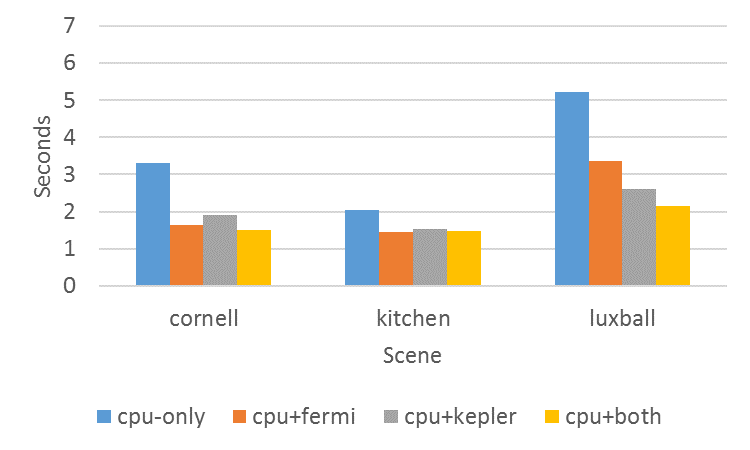
\includegraphics[width=\linewidth]{profiling/starpu_sched_peager}
    \caption{peager \label{fig:prof:starpu_sched_peager}}
  \end{subfigure}%
  \begin{subfigure}{.5\textwidth}
    \centering
    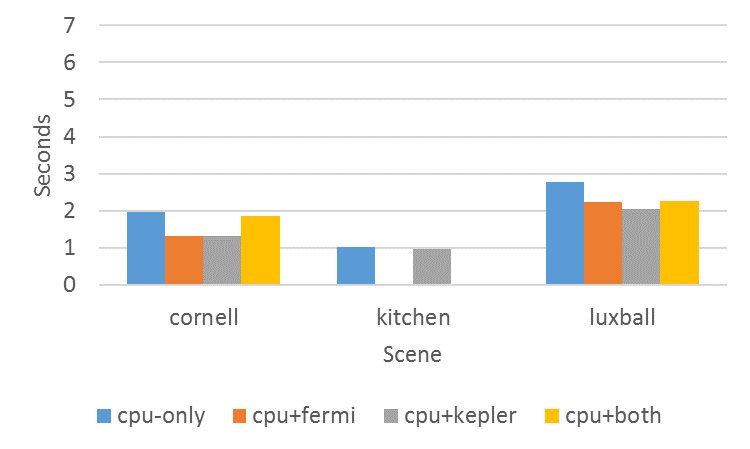
\includegraphics[width=\linewidth]{profiling/starpu_sched_pheft}
    \caption{pheft \label{fig:prof:starpu_sched_pheft}}
  \end{subfigure}
  \begin{subfigure}{.5\textwidth}
    \centering
    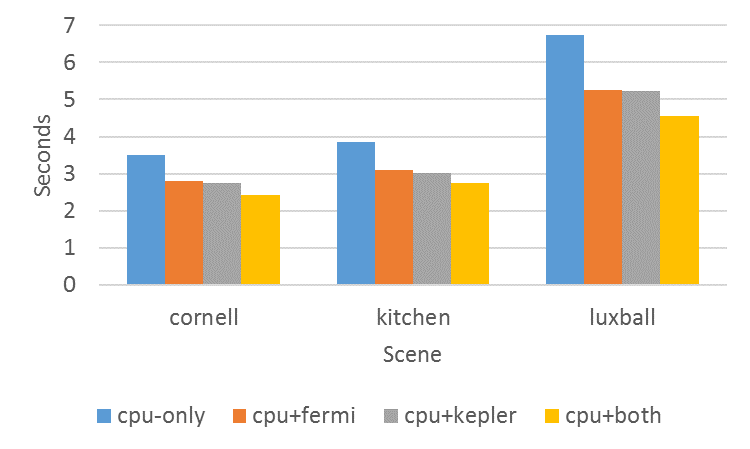
\includegraphics[width=\linewidth]{profiling/starpu_sched_dm}
    \caption{dm \label{fig:prof:starpu_sched_dm}}
  \end{subfigure}%
  \begin{subfigure}{.5\textwidth}
    \centering
    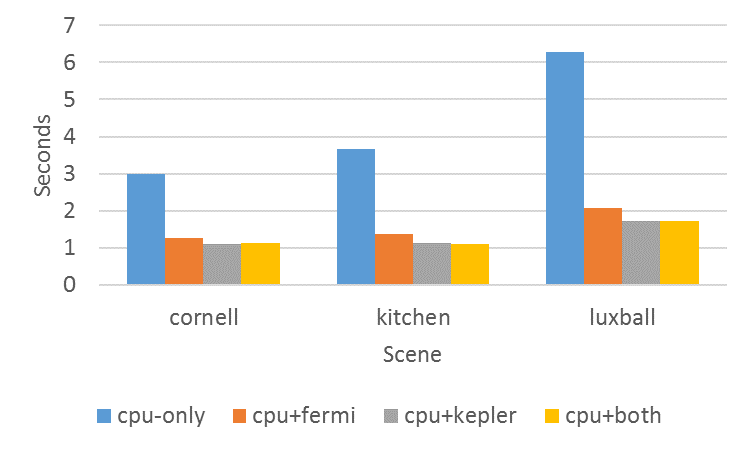
\includegraphics[width=\linewidth]{profiling/starpu_sched_dmda}
    \caption{dmda \label{fig:prof:starpu_sched_dmda}}
  \end{subfigure}
  \caption{Speedup of the different schedulers by successfully adding new devices \label{fig:prof:starpu_scheds}}
\end{figure}

One of the most importants aspects to analyze was how the chosen scheduler impacts performance.

\subsection{Overall Performance Comparison}

The best case scenario for each possible approach is shown in \cref{fig:prof:overall}. This serves to show the impact of \starpu with each different scheduler against framework-less solutions.

\begin{figure}[!htp]
  \centering
  \begin{subfigure}{.5\textwidth}
    \centering
    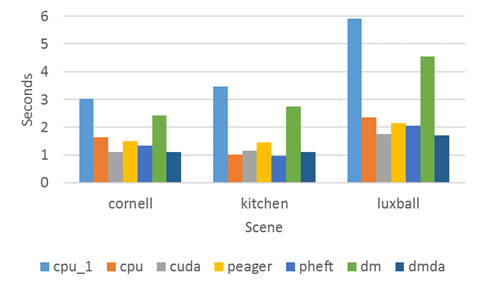
\includegraphics[width=\linewidth]{profiling/1iter_time}
    \caption{Avg. iteration time \label{fig:prof:overall_time}}
  \end{subfigure}%
  \begin{subfigure}{.5\textwidth}
    \centering
    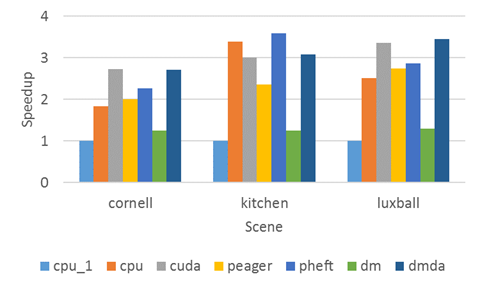
\includegraphics[width=\linewidth]{profiling/1iter_speedup}
    \caption{Speedup \label{fig:prof:overall_speedup}}
  \end{subfigure}
  \caption{Best cases for each different implementation and scheduler \label{fig:prof:overall}}
\end{figure}

\subsection{Concurrent Iterations}

With the employed approach, task-level parallelism is limited. The \textbf{dmda} does not support combined workers, greatly lowering efficiency of \cpu tasks. \textbf{pheft} does support this, but its not a data aware scheduler, meaning that data transfers are not considered when assigning tasks. As a result, performance with \starpu is limited when using processing a single iteration.

\todo{mudar isto para speedup e por legenda}
\image[width=0.5\textwidth]{profiling/iters_at_once_both}{Speedup with concurrent iterations}{fig:prof:iters_at_once_both}

By using concurrent iterations, however, extra speedups can be achieved, as shown in \cref{fig:prof:iters_at_once_both}.

\end{document}
